

屋内環境における位置推定において,ユーザの3次元的な位置,特に現在いる階層の把握が必要となる.
PDRによる2次元軌跡推定では,ユーザの水平面上の移動は追跡できるものの,階層間の移動の検知は難しく,
特に複数階層を有する大規模な商業施設やオフィスビルでの屋内ナビゲーションにおいて大きな課題となる.

この課題に対し,これまでに様々なアプローチが提案されている.
Wi-Fiアクセスポイントの電波強度やBluetoothビーコンを利用する手法は既存のインフラを活用できる一方で,
電波強度が壁や人の移動の影響を受けやすく,各階での適切な配置が必要となる.
QRコードやARマーカーを用いる手法は高精度な階層識別が可能だが,
ユーザが意図的にマーカーをスキャンする必要があり,継続的な階層検知には適していない.
近年では,機械学習を用いて加速度センサやジャイロセンサのデータから階段の昇降を検知する手法も提案されている.
このアプローチは階段の昇降動作を高精度に検知できる一方で,エレベーターでの移動は検知できず,
また十分なデータセットによる訓練が必要となる.

本手法では気圧センサのデータを利用し,PDRによる2次元軌跡推定に垂直方向の移動検知を組み合わせた
3次元位置推定を行う.気圧センサは標準的なスマートフォンに搭載されており,
追加のインフラやハードウェアを必要としない.気圧は高度に応じて変化するため,
屋内環境においても階層の識別と移動検知が可能であり,
ユーザの明示的な操作を必要とせずエレベーターや階段での移動も追跡できる.

しかし,気圧データを用いた階層検知には,センサ自体のノイズや量子化誤差による変動,
気象条件による外気圧の変動,エレベーターや階段移動時の急激な気圧変化,
さらに建物内の空調システムによる局所的な気圧変化といった課題が存在する.
これらの課題に対処するため,本研究では安定区間検出とクラスタリングを組み合わせた
2段階の手法を提案する.以下,各段階について詳細に説明する.



\subsection{安定区間の検出}
気圧データから信頼性の高い階層情報を抽出するためには,まず安定した気圧値が観測される期間を特定する必要がある.
ここでの安定区間とは,一定時間以上にわたって気圧の変動が小さい期間を指す.
安定区間の検出では,気圧変動の閾値として0.02 hPa(約1.7mの高度差に相当)と,最小継続時間として4秒という
パラメータを用いる.

安定区間の検出では,指定された時間幅のウィンドウを用いて気圧データを走査する.
各ウィンドウ内での気圧の最大値と最小値の差が閾値以下である場合,そのウィンドウを安定区間として記録する.
この手法により,短期的なノイズの影響を受けにくい安定した気圧値を抽出することができる.

\begin{figure}[h]
	\centering
	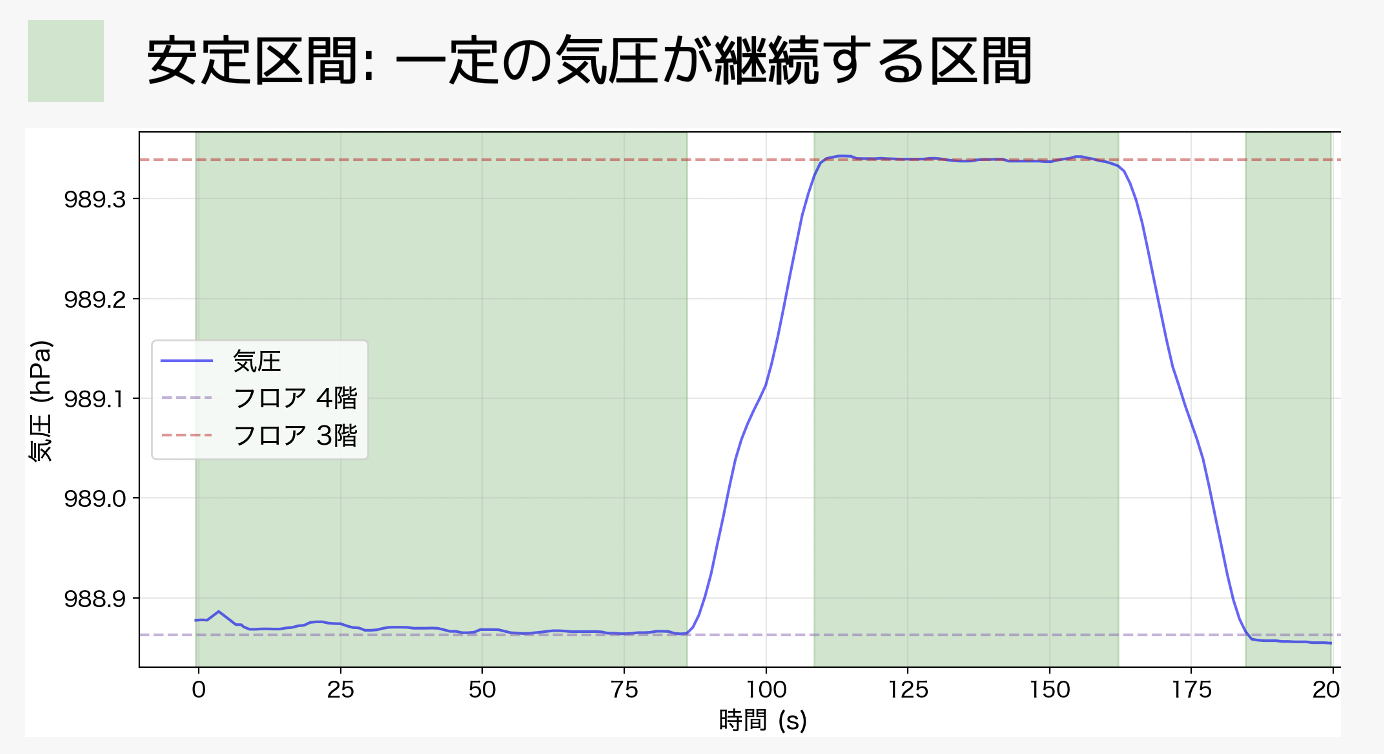
\includegraphics[width=\linewidth]{image/stable.jpg}
	\caption{安定歩行区間の検出}    \label{fig:stable_section}
\end{figure}

\subsection{DBSCANによる階層のグルーピング}
検出された安定区間内の気圧値に対して,DBSCANアルゴリズムを適用し階層のグルーピングを行う.
DBSCANは,クラスタ数を事前に指定する必要がなく建物の階数が未知の場合でも適用可能である.
また,ノイズの影響を受けにくく外れ値を自動的に除外できる特徴を持つ.
さらに,気圧値の分布が正規分布に従わない場合でも,任意の形状のクラスタを検出可能という利点がある.

DBSCANのパラメータは,建物の物理的特性に基づいて設定する.
具体的には,標準大気圧の高度による変化(約12 Pa/m)と標準的な階高(3.0 m)を考慮する.
クラスタ半径$\epsilon$は標準階高の半分の高度変化に相当する0.018 hPaとし,
最小サンプル数$minPts$は1と設定する.

クラスタリングにより得られた各グループの平均気圧値を計算し,これを階層の代表値として採用する.
その後,気圧値の大きさに基づいて階層番号を割り当てる.
具体的には,最も気圧値が大きい(最も低層の)クラスタから順に0から始まる整数値を割り当てる.
これにより,建物の物理的な構造と整合性のある階層番号付けが実現できる.

\subsection{階層間遷移の検知}
階層間の移動は,安定区間の間に観測される顕著な気圧変化として検出される.
本手法では,連続する安定区間の間の気圧の変化パターンを分析することで,
階層間の移動を検知する.

階層間の遷移検知において,まず時系列データ内で1.0秒以上の間隔が空いている箇所を特定し,
それを境界として異なる時間区間に分割する.次に,各時間区間について,
その区間内の気圧値に対応する軌跡データを抽出する.
最後に,抽出された軌跡データとDBSCANにより特定された階層の気圧範囲を照合することで,
各時間区間における階層を特定する.この手法により,エレベーターや階段による移動,
さらには一時的な滞在を含む複雑な移動パターンも適切に検出することが可能となる.

\subsection{適用例}
本手法を実データに適用した例を図\ref{fig:move_between_floor}に示す.
この例では,気圧データから複数の階層が識別され,
それぞれの階層における滞在時間と移動の様子が明確に可視化されている.
気圧データの分析から,各階層を代表する気圧値が物理的に妥当な間隔で分離されており,
階層間の移動が連続的な気圧変化として捉えられていることが確認できる.
また,各階層での滞在時における気圧値の安定性も明確に示されている.

特に注目すべき点として,安定区間の検出とDBSCANによるグルーピングを組み合わせることで,
センサノイズや一時的な気圧変動に影響されることなく,信頼性の高い階層識別が
実現できていることが挙げられる.この結果は,提案手法が実環境における
3次元位置推定に有効であることを示している.


\begin{figure}[h]
	\centering
	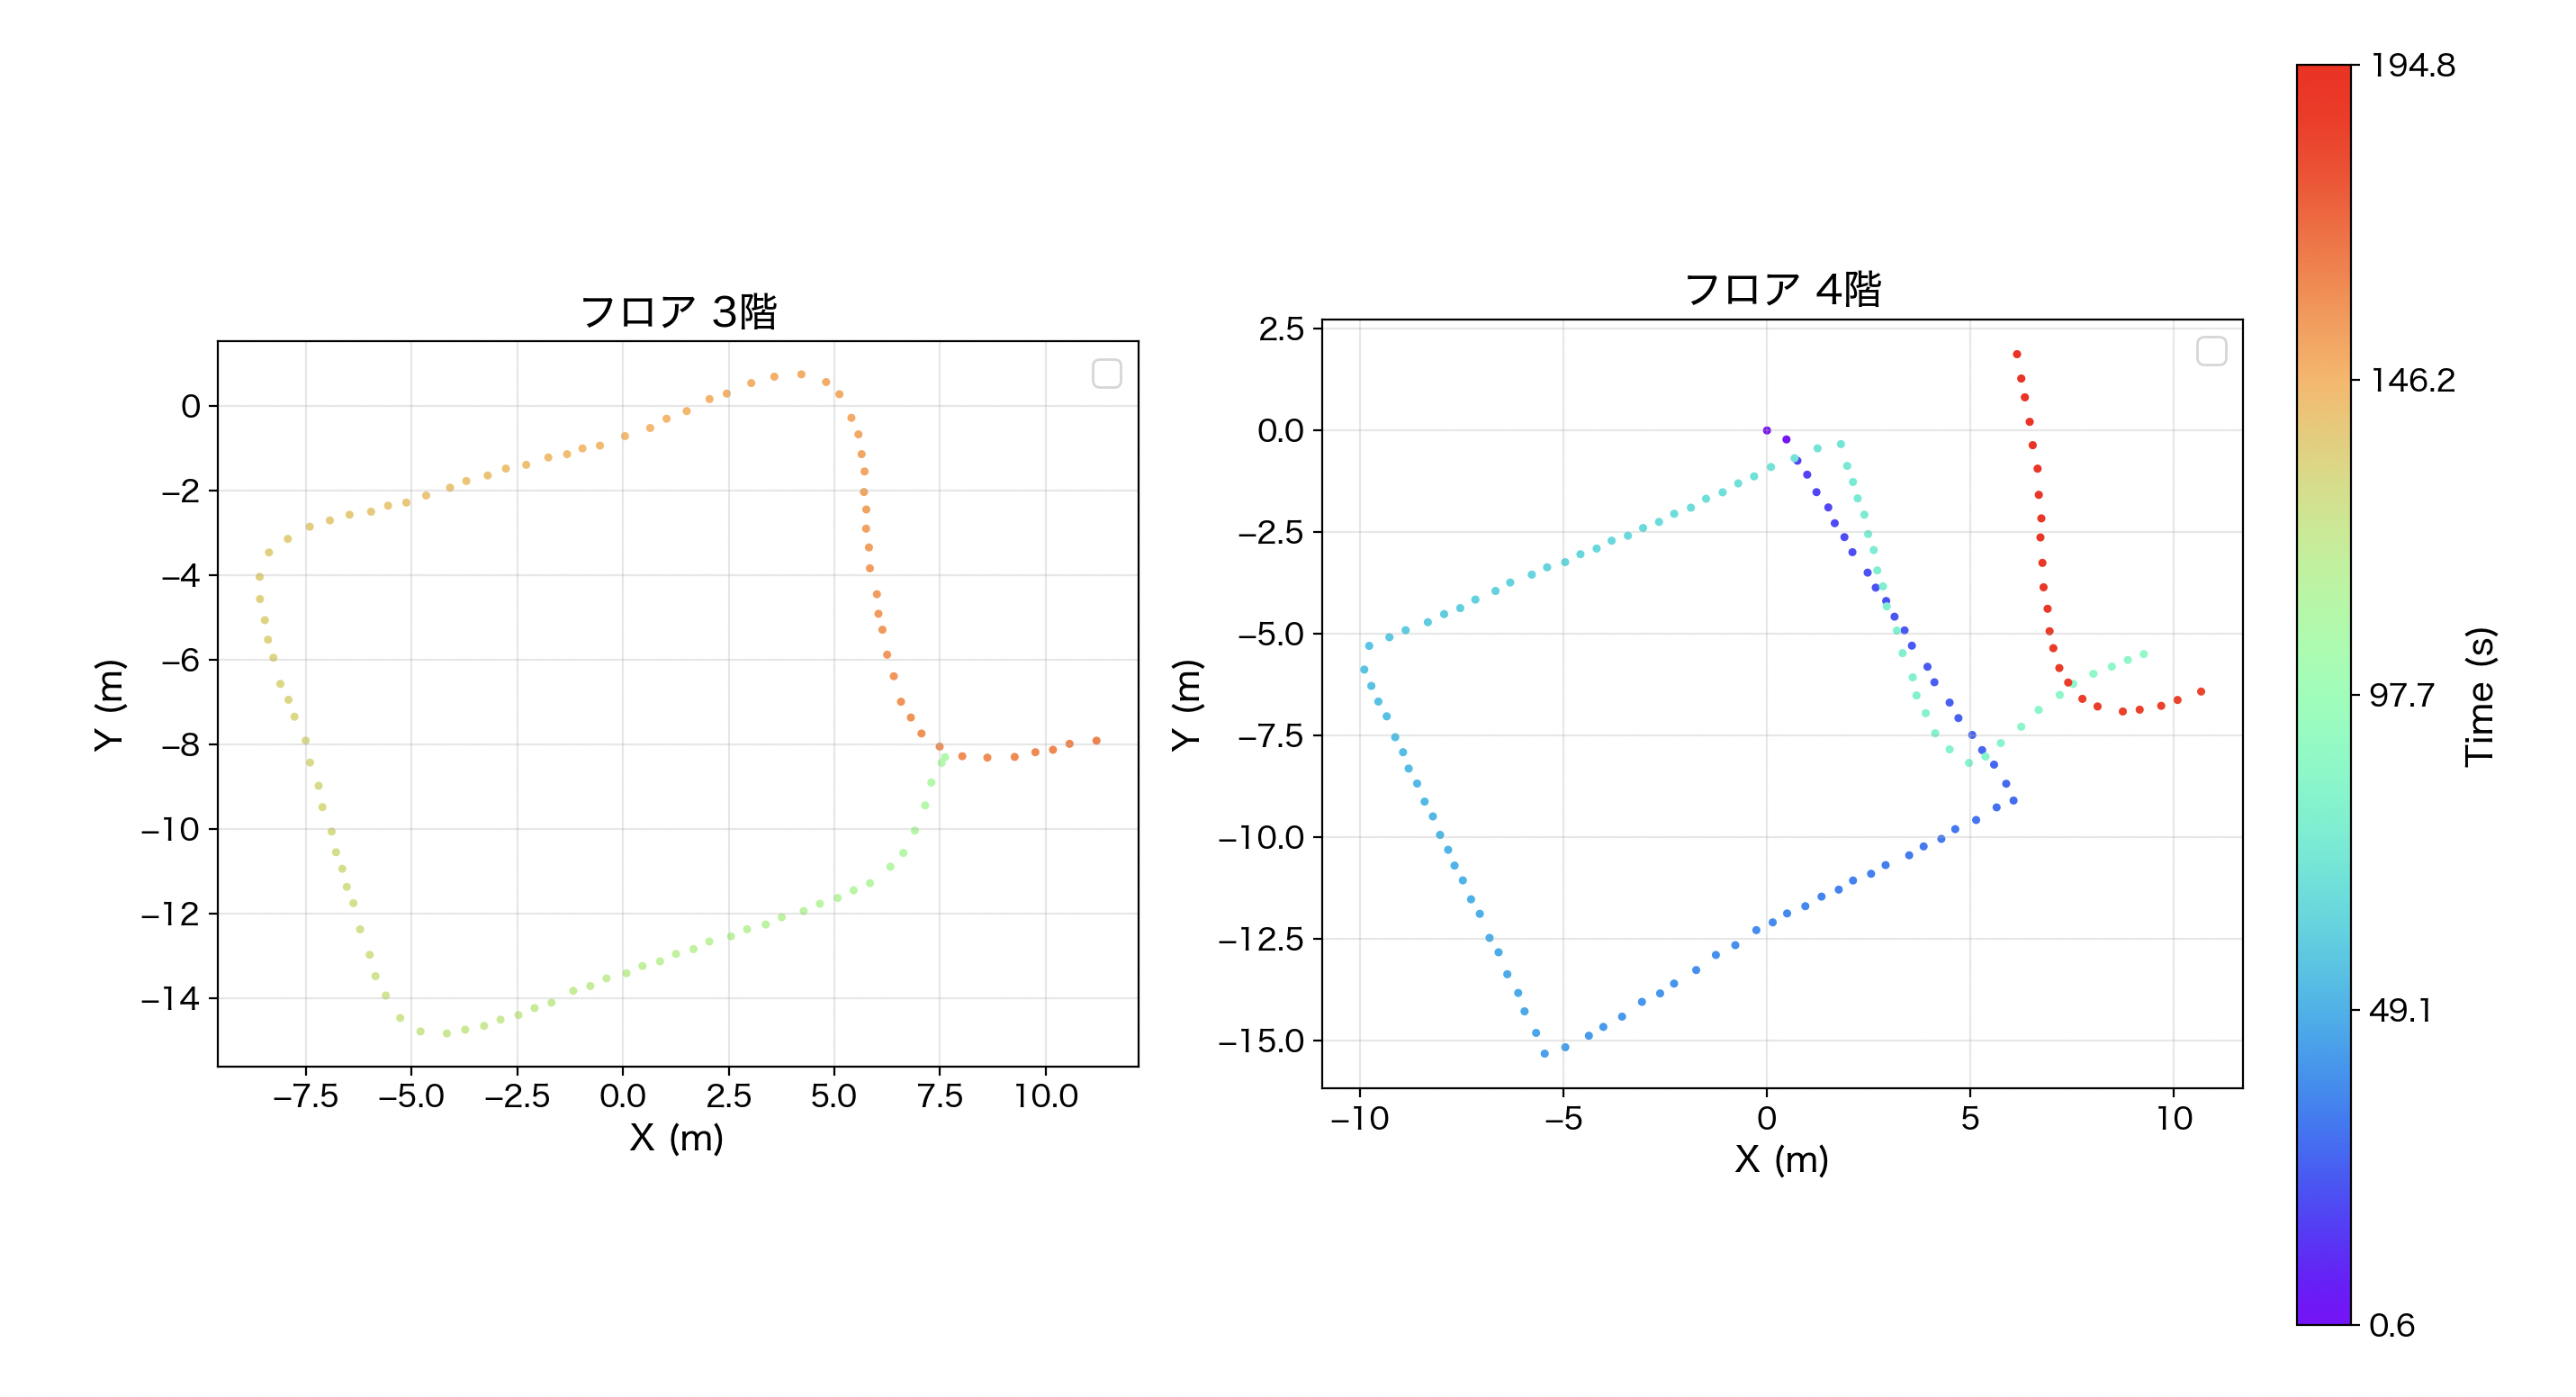
\includegraphics[width=\linewidth]{image/move_between_floor.jpg}
	\caption{適用例}    \label{fig:move_between_floor}
\end{figure}
